\documentclass{beamer}
\title{Unidad 13: Polimorfismo}
\date[today]{\today}
\author[Name]{CS1102 – PROGRAMACIÓN ORIENTADA A OBJETOS 1 
CICLO 2019-2}
\institute[Department]{UTEC}

\usetheme{lumc}
\usepackage{multicol} % 
%\usepackage{animate}  % animation
\usepackage{amsmath,amsfonts,amssymb} 
\usepackage{listings}
\usepackage{hyperref}

\usepackage[style=verbose,backend=biber]{biblatex}
\addbibresource{b1.bib}

\lstset{basicstyle=\ttfamily,breaklines=true}

\newcommand{\estilocpp}{
\lstset{
    language=C++,
    basicstyle=\fontsize{15}{20}\ttfamily\ttfamily,
    keywordstyle=\color{jpurple}\bfseries,
    stringstyle=\color{red},
    commentstyle=\color{verde},
    morecomment=[s][\color{blue}]{/**}{*/},
    extendedchars=true,
    showspaces=false,
    showstringspaces=false,
    numbers=left,
    numberstyle=\normalsize,
    breaklines=true,
    backgroundcolor=\color{cyan!10},
    breakautoindent=true,
    captionpos=b,
    xleftmargin=0pt,
    tabsize=2
}}

\begin{document}

\begin{frame}
\titlepage
\end{frame}


%%%%%%%%%%%%%%%%%%%%%%%%%%%%%%%%%%%%%%%%%%%%%%%%%%
\section{Logros de la Sesión}
%%%%%%%%%%%%%%%%%%%%%%%%%%%%%%%%%%%%%%%%%%%%%%%%%%

\begin{frame}[fragile]{Logros de la sesión}
    \begin{itemize}[<+- | alert@+>]
        \item Al finalizar la sesión los alumnos entienden el concepto de polimorfismo
        \item Conoceran los distintos tipos de Polimorfismo soportado en el lenguaje C++.
        \item Conocerán las relaciones entre el Polimormismo y otros tipos de abstracción en el lenguaje.
        \item Utiliza el polimorfismo para representar comportamiento dinámico en C++
    \end{itemize}
\end{frame}


%%%%%%%%%%%%%%%%%%%%%%%%%%%%%%%%%%%%%%%%%%%%%%%%%%
\section{Motivación}
%%%%%%%%%%%%%%%%%%%%%%%%%%%%%%%%%%%%%%%%%%%%%%%%%%


\begin{frame}[fragile]{¿Quien es Morfeo?}
\frametitle{Polimorfismo}
\begin{itemize}
  ¿Quien puede adoptar la forma de cualquier humano?
\end{itemize}

\begin{figure}
\centering
\begin{minipage}{.45\textwidth}
\centering

\includegraphics[width=.7\linewidth]{poli/morfeo-precuela.jpg}
\caption{Morfeo de Matrix}
\end{minipage}
\begin{minipage}{.45\textwidth}
\centering
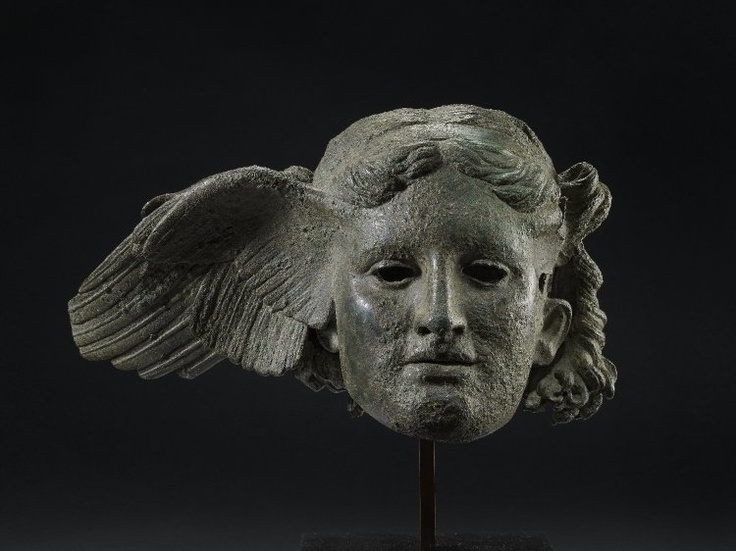
\includegraphics[width=.7\linewidth]{poli/morfeo1.jpg}
\caption{Dios griego Morfeo}
\end{minipage}
\caption{Una entidad multiples formas}
\end{figure}
\end{frame}


\begin{frame}[fragile]{¿Polimorfismo en biología?} 
\begin{figure}
\centering
\begin{minipage}{.9\textwidth}
\centering
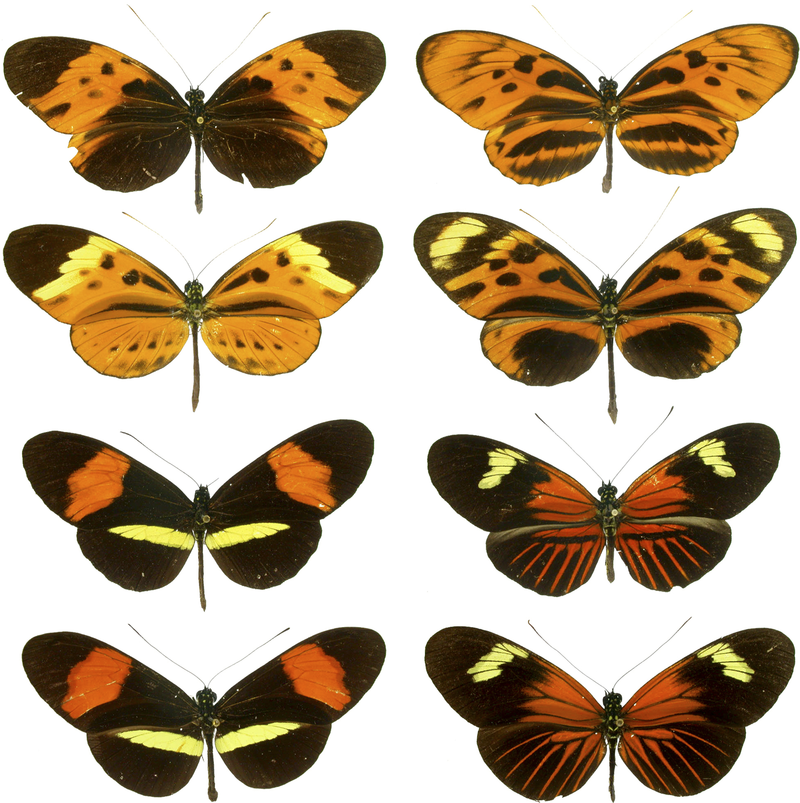
\includegraphics[width=.45\linewidth]{poli/Heliconius_mimicry.png}
\caption{Lepidoptera}
\end{minipage}
\caption{¿Es la misma especie o especies diferentes?}
\end{figure}

\end{frame}


%%%%%%%%%%%%%%%%%%%%%%%%%%%%%%%%%%%%%%%%%%%%%%%%%%
\section{Adquisición}
%%%%%%%%%%%%%%%%%%%%%%%%%%%%%%%%%%%%%%%%%%%%%%%%%%

\begin{frame}[fragile]{¿Que es el Polimorfismo en la programación?}

    \begin{itemize}
        \item Polimorfismo significa que una entidad puede tomar muchas formas.
        \item En la programación convencional cada valor o variable puede ser de un solo tipo y valor. Esto se conoce como monomorfo. 
        \item En lenguajes que soportan polimorfismo, un objeto polimórfico es una entidad, como una variable o argumento de función, que puede tener valores de tipos diferentes en el curso de ejecución. 
        \item Las funciones polimórficas son funciones que tienen argumentos polimórficos.
        \item Los tipos polimórficos son tipos cuyas operaciones son aplicables a valores de más de un tipo. 
    \end{itemize}


\end{frame} 

%%%%%%%%%%%%%%%%%%%%%%%%%%%%%%%%%%%%%%%%%%%%%%%%%%


\begin{frame}[fragile]{Clasificación del Polimorfismo(1)}

\begin{figure}
\centering
\begin{minipage}{.9\textwidth}
\centering
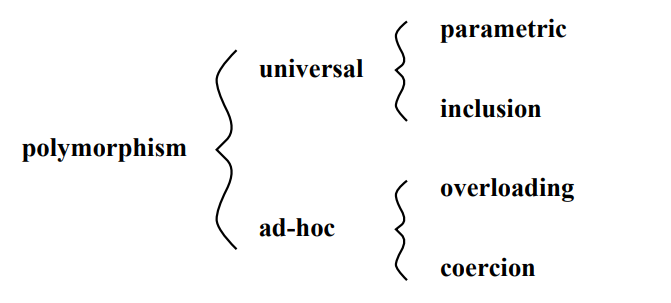
\includegraphics[width=.7\linewidth]{poli/clasipoli.png}
\caption{Clasificación del Polimorfismo}\cite{Cardelli1985}

\end{minipage}

\end{figure}

\end{frame}  


%%%%%%%%%%%%%%%%%%%%%%%%%%%%%%%%%%%%%%%%%%%%%%%%%%


\begin{frame}[fragile]{Clasificación del Polimorfismo(2)}

    \begin{itemize}
        \item El polimorfismo A) universal se divide en: 1) \textbf{parametric}, el cual se obtiene cuando una función funciona de manera uniforme en una variedad de tipos: estos tipos normalmente exhiben alguna estructura común.

        \item Por otra parte 2)  \textbf{inclusion} se refiere a la herencia y los subtipos. (Visto en las clases de Herencia)

        \item  El polimorfismo B) \textbf{ad-hoc} o no universal, se obtiene cuando una función trabaja, o parece funcionar, con varios tipos diferentes (que pueden no exhibir una estructura común) y pueden comportarse en formas no relacionadas para cada tipo.

        \item También hay dos tipos principales de polimorfismo ad-hoc. El 3)\textbf{overloading} el mismo nombre de variable esto se usa para denotar diferentes funciones, y el contexto se usa para decidir qué función se denota mediante un instancia particular del nombre.

        \item Y 4) \textbf{coercion} es, en cambio, una operación semántica que se necesita para convertir un argumento para el tipo esperado por una función, en una situación que de lo contrario resultaría en un error de tipo.

        \item En el caso del polimorfismo universal, uno puede afirmar con confianza que algunos valores (es decir, funciones polimórficas) tienen muchos tipos, mientras que en el polimorfismo ad-hoc esto es más difícil de sostener, ya que uno puede tomar la posición de que una función polimórfica ad-hoc es realmente un pequeño conjunto de funciones monomórficas.\shortcites{Cardelli1985}

    \end{itemize}


\end{frame}  


%%%%%%%%%%%%%%%%%%%%%%%%%%%%%%%%%%%%%%%%%%%%%%%%%%


\begin{frame}[fragile]{Los 4 tipos de Polimorfismo en C++}

    \begin{itemize}
        \item De los 4 tipos de polimorfismo, ¿como se pueden representar en C++?

         \item  1) \textbf{parametric}, es conocido como \textbf{compile-time polymorphism}.

        \item 2)  \textbf{inclusion} se refiere a \textbf{runtime polymorphism} o \textbf{subtype} herencia de tipos.


        \item El 3)\textbf{overloading} lleva el mismo nombre.

        \item Y 4) \textbf{coercion} es, conocido como (implicito o explicito) \textbf{casting}.


    \end{itemize}


\end{frame}  



%%%%%%%%%%%%%%%%%%%%%%%%%%%%%%%%%%%%%%%%%%%%%%%%%%

\begin{frame}[fragile]{1) Parametric o Compile-Time Polymorphism}

 \begin{itemize}
        \item Provee un medio para ejecutar el mismo código para cualquier tipo. En C++ esto se implementa vía plantillas.

\end{itemize}

  \estilocpp
  \begin{lstlisting}[frame = single]
#include <iostream>
#include <string>

  template <class T>
  T max(T a, T b) {
    return a > b ? a:b;
  }

  int main() {
    std::cout << ::max(9, 6) << "\n";
    std::cout << ::max(12.6, 3.0) << "\n";
    return 0;
  }

  \end{lstlisting}
  \caption{¿Con que tipos de datos funciona la función max?}
\end{frame}  

%%%%%%%%%%%%%%%%%%%%%%%%%%%%%%%%%%%%%%%%%%%%%%%%%%


\begin{frame}[fragile]{2) Inclusion o Subtype Polymorphism (1)}

 \begin{itemize}
        \item Es lo que conocemos como el uso de clases derivadas vía punteros y referencias. También llamado Runtime Polymorphism.

        \item En el siguiente ejemplo usamos una relación de clases para la familia de felinos.

\end{itemize}

  \estilocpp
  \begin{lstlisting}[frame = single]
  class Felino {
    public:
      virtual void maullido() = 0;
  };

  class Gato: public Felino {
    public:
      void maullido() {
        std::cout << "Maullido como un gato\n";
      }
  }

  class Tigre: public Felino {
    public:
      void maullido() {
        std::cout << "Maullido como un tigre!!\n";
      }
  }
  ...

  \end{lstlisting}

\end{frame}  


%%%%%%%%%%%%%%%%%%%%%%%%%%%%%%%%%%%%%%%%%%%%%%%%%%


\begin{frame}[fragile]{2) Inclusion o Runtime o Subtype Polymorphism(2)}

 \begin{itemize}
        \item Veamos ahora un programa que usa la jerarquía de clases de Felinos.
\end{itemize}

  \estilocpp
  \begin{lstlisting}[frame = single]

#include <iostream>
#include "felinos.h"

void do_maullido(Felino *gato) {
  gato->maullido();
}

int main() {
  
  Gato gato;
  Tigre tigre;
  Puma puma;
  do_maullido(&gato);
  do_maullido(&tigre);  
  do_maullido(&puma);  
}
\end{lstlisting}
   \begin{itemize}
    \item ¿Que resultado dará la llamada a la función?
    \item ¿En que momento se determina el tipo correspondiente del parámetro?
  \end{itemsize}
\end{frame}  


%%%%%%%%%%%%%%%%%%%%%%%%%%%%%%%%%%%%%%%%%%%%%%%%%%

\begin{frame}[fragile]{3) Overloading o Sobrecarga}

 \begin{itemize}
        \item Esto permite tener varias funciones con el mismo nombre que se comportan diferente de acuerdo al tipo de dato que reciben.
        \item Por ejemplo la función suma con parámetros enteros y con cadenas.
\end{itemize}

  \estilocpp
  \begin{lstlisting}[frame = single]
#include <iostream>
#include <string>
using namespace std;
int add(int a, int b) {
 return a + b;
}
std::string add(string a, string b) {
 std::string result(a);
 result += b;
 return result;
}

int main() {
 std::cout << add(5, 9) << "\n";
 std::cout << add("hello ", "world") << "\n";
}
  \end{lstlisting}

\begin{itemize}
        \item ¿Que resultado se obtiene?
\end{itemize}
\end{frame}  

%%%%%%%%%%%%%%%%%%%%%%%%%%%%%%%%%%%%%%%%%%%%%%%%%%

\begin{frame}[fragile]{4) Coercion o Casting (1)}

 \begin{itemize}
        \item Casting o conversión ocurre cuando un objeto o variable es convertido a otro tipo de objeto o tipo de dato.
        \item Por ejemplo una variable entera asignada por un valor real implicitamente se convierte a entero el valor real.
\end{itemize}

  \estilocpp
  \begin{lstlisting}[frame = single]

float b = 6; 
int a = 9.99;

int x = (int) 3.1415;

\end{lstlisting}
\end{frame}  

%%%%%%%%%%%%%%%%%%%%%%%%%%%%%%%%%%%%%%%%%%%%%%%%%%

\begin{frame}[fragile]{4) Coercion o Casting (2)}

 \begin{itemize}
        \item La coerción también ocurre si el constructor de una clase no se establece de forma explícita.
\end{itemize}

  \estilocpp
  \begin{lstlisting}[frame = single]
#include "tipos.h"
class Alumno {
    entero nota1, nota2;
    caracter* name;
public:
    Alumno(entero i) { };
    Alumno(const caracter* n, entero j = 0) { };
};

void add(Alumno) { };

int main() {

    Alumno obj1 = 2; // obj1 = Y(2)

    Alumno obj2 = "somestring"; // obj1 = Y(2)

    obj1 = 10;   // obj1 = Y(10)

    add(5);   // add(Y(5))
}

\end{lstlisting}

  \begin{itemize}
    \item ¿Se puede evitar?
  \end{itemsize}
\end{frame}  


%%%%%%%%%%%%%%%%%%%%%%%%%%%%%%%%%%%%%%%%%%%%%%%%%%
\section{Transferencia}
%%%%%%%%%%%%%%%%%%%%%%%%%%%%%%%%%%%%%%%%%%%%%%%%%%

\begin{frame}[fragile]{Ejercicio 1}
  \begin{block}{Enunciado}
  Escribir un algoritmo en C++ que construya una clase Array Polimórfico de tipo \textbf{paramétrico} usando plantillas que permita crear un arreglo de cualquier tipo de dato:
  \begin{itemize}
      \item Construya un Array de enteros e inicialicelos. 
      \item Construya una función que imprima los datos almacenados.
  \end{itemize}

    \estilocpp
  \begin{lstlisting}[frame = single]

template <typename T> 
class Array { 
private: 
    T *ptr; 
    int size; 
public: 
    Array(T arr[], int s); 
    void print(); 
};

\end{lstlisting}
  
\end{block}   
\end{frame} 


\begin{frame}[fragile]{Ejercicio 1 (Solución)}

\estilocpp
  \begin{lstlisting}[frame = single]

#include <iostream> 
using namespace std; 

template <typename T> 
class Array { 
private: 
  T *ptr; 
  int size; 
public: 
  Array(T arr[], int s); 
  void print(); 
}; 

template <typename T> 
Array<T>::Array(T arr[], int s) { 
  ptr = new T[s]; 
  size = s; 
  for(int i = 0; i < size; i++) 
    ptr[i] = arr[i]; 
} 

 
\end{lstlisting}  
\end{frame} 


\begin{frame}[fragile]{Ejercicio 1 (Solución)}
\estilocpp
  \begin{lstlisting}[frame = single]
template <typename T> 
void Array<T>::print() { 
  for (int i = 0; i < size; i++) 
    cout<<" "<<*(ptr + i); 
  cout<<endl; 
} 
int main() { 
  int arr[5] = {1, 2, 3, 4, 5}; 
  Array<int> a(arr, 5); 
  a.print(); 
  return 0; 
} 

\end{lstlisting}
   
\end{frame} 

%%%%%%%%%%%%%%%%%%%%%%%%%%%%%%%%%%%%%%%%%%%%%%%%%%
\begin{frame}[fragile]{Ejercicio 2}
  \begin{block}{Enunciado}
\begin{itemsize}
\item Diseñe un algoritmo en C++ que use polimorfismo de (\textbf{inclusion}) o subtipo.El programa debe representar la jerarquía de clases para una imagen y sus clases derivadas JPG y PNG.
\end{itemsize}
\estilocpp
\begin{lstlisting}[frame = single]
class Imagen {
private:
    entero alto;
    entero ancho;
public:
    Imagen(entero _alto, entero _ancho):alto{_alto}, ancho{_ancho} {}
    virtual void guardar(const string &Nombre) = 0;
};
class JPEG : public Imagen {
public:
    JPEG(entero _alto, entero _ancho):Imagen(_alto, _ancho){}
    void guardar(const string &Nombre) override ;
};
class PNG: public Imagen {
public:
    PNG(entero _alto, entero _ancho):Imagen(_alto, _ancho){}
    void guardar(const string &Nombre) override ;
};
\end{lstlisting}
\end{block}
\end{frame} 

%%%%%%%%%%%%%%%%%%%%%%%%%%%%%%%%%%%%%%%%%%%%%%%%%%
\begin{frame}[fragile]{Ejercicio 2 (Solución)}
\estilocpp
\begin{lstlisting}[frame = single]
void PNG::guardar(const string &Nombre) {
    std::cout << "Guardando un archivo PNG " << Nombre;
}
void JPEG::guardar(const string &Nombre){
    std::cout << "Guardando un archivo JPEG" << Nombre;
}

void guardarImagen(Imagen *img, const string &Nombre)
{
    img->guardar(Nombre);
}

int main() {

    JPEG jpg(10, 20);
    PNG png(30, 30);
    string Nombre1 = "rombo.jpg";
    string Nombre2 = "cubo.png";
    guardarImagen(&jpg, Nombre1);
    guardarImagen(&png, Nombre2);
}
\end{lstlisting}
\end{frame} 

%%%%%%%%%%%%%%%%%%%%%%%%%%%%%%%%%%%%%%%%%%%%%%%%%%

\begin{frame}[fragile]{Ejercicio 3}
\begin{block}{Enunciado}
\begin{itemsize}
\item Escribir un programa en C++ que use sobrecarga(\textbf{overloading}). 
\item Dos físicos quieren saber cual es el diametro de una pompa de jabón cuando se junta en el aire con otra. Para ello se necesitan sobrecargar un operador de suma y asignación. 
\item La sobrecarga de operadores es equivalente a la sobrecarga de una función, en este caso se sobrecarga el operador +=. 
\item Realice la simulación y ejecute una operación de suma de pompas de jabón. 
\end{itemsize}

\estilocpp
\begin{lstlisting}[frame = single]

#include "Tipos.h"
class Pompa {
  private:
    real radio;
  public:
    Pompa();
};

\end{lstlisting}
\end{block}
\end{frame} 

%%%%%%%%%%%%%%%%%%%%%%%%%%%%%%%%%%%%%%%%%%%%%%%%%%

\begin{frame}[fragile]{Ejercicio 3 (Solución)}
\begin{itemsize}
\item \href{http://bit.ly/33h9e0d}{http://bit.ly/33h9e0d}
\end{itemsize}

\estilocpp
\begin{lstlisting}[frame = single]

#include "Tipos.h"
class Pompa {
  private:
    real radio;
  public:
    Pompa();
    Pompa(real pradio):radio{pradio}{}
    void setRadio(real pradio){radio = pradio;}
    real Diametro() const {return radio*2;}
    real Radio() const {return radio;}

    Pompa& operator+=(Pompa z){radio+=z.Radio(); return *this;}
};
int main(){
  Pompa p1(10);
  Pompa p2(15);
  p1 += p2;
  std::cout << p1.Diametro();
}

\end{lstlisting}
\end{frame} 

%%%%%%%%%%%%%%%%%%%%%%%%%%%%%%%%%%%%%%%%%%%%%%%%%%
\begin{frame}[fragile]{Ejercicio 4}
\begin{block}{Enunciado}
\begin{itemsize}
\item Construya una clase Persona en los que se observe el casting por constructor.
\end{itemsize}
\estilocpp
\begin{lstlisting}[frame = single]
class Persona {
private:
    real peso;
    entero edad;
    caracter* nombre;
public:
    Persona(entero _edad):edad{_edad}, peso{0.0}, nombre{""} {}
    Persona(caracter * _nombre):edad{0}, peso{0}, nombre{_nombre}{}
    void print(){std::cout << "peso:" << peso << " edad:" << edad << "nombre:" << nombre; }
};
int main() {
    Persona p1 = 5;
    Persona p2 = "Juan";
    p1.print();
    p2.print();
}
\end{lstlisting}

\end{block}
\end{frame} 

%%%%%%%%%%%%%%%%%%%%%%%%%%%%%%%%%%%%%%%%%%%%%%%%%%
\section{Cierre}
%%%%%%%%%%%%%%%%%%%%%%%%%%%%%%%%%%%%%%%%%%%%%%%%%%

\begin{frame}[fragile]{Cierre}
  \begin{block}{En esta sesión aprendiste}
    \begin{itemsize}
      \item A conocer el concepto de comportamiento polimórfico. 
      \item A conocer la implementación en C++ de los distintos tipos de polimorfismo.

    \end{itemsize}
  \end{block}
\end{frame}


\end{document}